\section{Tighter GSD security} \label{sec:tighter-gsd-security}

In this section, we present the main theoretical result behind Theorem~\ref{theorem:treekem-security-informal} in Theorem~\ref{theorem:sdgsd-security}. To this end, we first define a modified version of the public-key GSD game from \cite{ttkem} and then proceed to prove Theorem~\ref{theorem:sdgsd-security} in detail.

\subsection{Seeded GSD with Dependencies} \label{sec:sd-gsd-game}

\todo{Allow adversary to adaptively create nodes and seed dependencies.
	\begin{itemize}
		\item adapt proofs to guess from $[N]$ as opposed to $[n]$
		\item handle case where $\qs$ triggered because adversary queried a seed and that seed later became the seed of a newly created safe node
	\end{itemize}
}

The GSD game defined here is inspired by the definition of the public-key GSD game (Definition 7) and the proof of Theorem 3 in \cite{ttkem}. We have already motivated the differences in Section~\ref{sec:gsd-intro}. We will call our adapted game \emph{Seeded GSD with Dependencies} (SD-GSD). A very similar definition appears in \cite{modular-group-messaging}, providing essentially the same abstraction over TreeKEM and also allowing for an adversary to provide the randomness used for encryption and key generation. However, our definition has one notable difference: when asking to be challenged on a node with seed $s$, the adversary must distinguish $\hdep(s)$ from random as opposed to $s$. This stays true to how the group key is computed in TreeKEM and has the significant advantage of greatly simplifying our proof. On the other hand, the security implied by our definition is weaker (at least in the ROM), as it only guarantees that an adversary cannot compute the seed of the challenge node, whereas the other definitions guarantee that this seed cannot be distinguished from random.

\begin{definition}[The SD-GSD game] \label{def:sd-gsd-game}
	Let $\Pi = (\gen, \enc, \dec)$ a public-key encryption scheme, where $\gen(1^\eta)$ uses $\rho(\eta)$ random bits and $\{0, 1\}^{\rho(\eta)}$ is a subset of the message space.
	Let $\fhgen = \{ \hgen^{(\eta)} \mid \eta \in \N\}, \fhdep = \{ \hdh^{(\eta)} \mid \eta \in \N\}$ families of functions with $\hgen^{(\eta)}, \hdep^{(\eta)} \colon \{0, 1\}^{\rho(\eta)} \to \{0, 1\}^{\rho(\eta)}$. We will write $\hgen \coloneqq \hgen^{(\eta)}, \hdep \coloneqq \hdep^{(\eta)}$ and $\rho \coloneqq \rho(\eta)$ if $\eta$ is clear from the context.
	Define the game $\game{(\Pi, \fhgen, \fhdep)}{\eta}{SD\text{-}GSD}(\adv)$ for an adversary $\adv$:
	\begin{enumerate}[1.]
		\item \label{def:sd-gsd-game-step-init} The adversary $\adv$ outputs $n \in \N$ and a list of dependencies $D = \{(a_{i}, b_{i})\}_{i=1}^m \subseteq [n]^2$. For each $v \in [n]$:
		      \begin{enumerate}[(i)]
			      \item \begin{itemize}
				            \item \textbf{Case $v = b_i$ for some $i$ ($v$ is the target of some dependency):} set $s_v = \hdep(s_{a_i})$.
				            \item \textbf{Otherwise:} sample $s_v \from \{0, 1\}^\rho$.
			            \end{itemize}
			            We call $s_v$ the \emph{seed} of the node $v$ and a tuple $(a, b) \in D$ a \emph{seed dependency}.
			      \item Compute $(pk_v, sk_v) = \gen(1^\eta, \hgen(s_v))$.
		      \end{enumerate}
		      Set $\mathcal{C} = E = \varnothing$. We call the directed graph $([n], E)$ a \emph{GSD graph} of \emph{size} $n$.
		\item $\adv$ may adaptively make the following queries:
		      \begin{itemize}
			      \item $\mathrm{reveal}(v)$ for $v \in [n]$: $\adv$ is given $pk_v$.
			      \item $\mathrm{encrypt}(u, v)$ for $u, v \in [n], u \neq v, (u, v) \notin E$: $(u, v)$ is added to $E$ and $\adv$ is given $c \from \enc_{pk_u}(s_v)$.
			      \item $\mathrm{corrupt}(v)$ for $v \in [n], v \notin \mathcal{C}$: $\adv$ is given $s_v$ and $v$ is added to $\mathcal{C}$. We call such a node $v \in \mathcal{C}$ \emph{corrupted}. All nodes not reachable from any corrupted node in the graph $([n], E \cup D)$ are \emph{safe} (while all other nodes are \emph{unsafe}) and we call their seeds \emph{hidden} (even if an unsafe node happens to have the same seed).
		      \end{itemize}
		\item $\adv$ outputs a node $v \in [n]$. We call $v$ the \emph{challenge node}. A bit $b \from \{0, 1\}$ is sampled and $\adv$ is given
		      \[
			      r = \begin{cases}
				      \hdep(s_v) & b = 0 \\
				      s          & b = 1
			      \end{cases},
		      \]
		      where $s \from \{0, 1\}^\rho$.\footnote{Note that (in general) $r$ is not a hidden seed, as (with overwhelming probability) it is not the seed of any node.} $\adv$ may continue to do queries as before.
		\item \label{def:sd-gsd-game-step-output} $\adv$ outputs a bit $b'$. The output of the game is defined to be $1$ if $b' = b$, and $0$ otherwise.
	\end{enumerate}

	We require an adversary playing the above game to adhere to the following:
	\begin{itemize}
		\item The challenge node is safe
		\item The challenge node is not the source of a seed dependency\footnote{Otherwise the adversary could learn the value of $\hdep$ on the seed of the challenge node by creating a seed dependency with the challenge node as the source and corrupting the target node.}
		\item Every node is the source and target of at most one seed dependency\footnote{If a node were the source node of multiple seed dependencies, then corrupting one target node would reveal the seeds of all target nodes. Additionally, the computation of seeds is not well-defined if a node is the target of multiple dependencies.}
		\item The graph $([n], E \cup D)$ is acyclic and without self-loops
	\end{itemize}
\end{definition}

It is interesting to note that previous definitions of the GSD game also included the following restrictions to the adversary:
\begin{itemize}
	\item The challenge node always remains a sink in $([n], E)$
	\item $\operatorname{reveal}$ is never queried on the challenge node
\end{itemize}
Our proof in the ROM does not require these restrictions. If $\hdep$ is modelled as a random oracle, then an encryption edge outgoing from the challenge node, or knowing its public key gives no advantage to $\adv$, as by the assumption of $\hdep$ being a random oracle the only way to learn information about $\hdep(s)$ is by querying $s$.

\begin{definition}[SD-GSD security]
	Let $\Pi, \fhgen$ and $\fhdep$ as in Definition~\ref{def:sd-gsd-game} above and let $t, \epsilon, N, \delta$ functions in $\eta$.
	The triple $(\Pi, \hgen, \hdep)$ is \emph{$(t, \epsilon, N, \delta)$-SD-GSD-secure} if for all $\eta$, for any adversary $\adv$ constructing a GSD graph of size at most $N(\eta)$ and indegree at most $\delta(\eta)$ and running in time $t(\eta)$ we have
	\begin{align*}
		\advantage{(\Pi, \fhgen, \fhdep)}{\eta}{SD\text{-}GSD}(\adv) \coloneqq 2 \cdot \left(\pr{\game{(\Pi, \fhgen, \fhdep)}{\eta}{SD-GSD}(\adv) = 1} - \frac{1}{2}\right) \le \epsilon(\eta).
	\end{align*}
\end{definition}

Since in this work we are interested in SD-GSD security for the case where $\hgen$ and $\hdep$ are modelled as random oracles and our focus is on the encryption scheme being used, we introduce the following definition for convenience.

\begin{definition}[SD-GSD security in the ROM]
	A public-key encryption scheme $\Pi$ is \emph{$(t, \epsilon, N, \delta)$-SD-GSD-secure in the ROM} if the triple $(\Pi, \fhgen, \fhdep)$ is $(t, \epsilon, N, \delta)$-SD-GSD-secure when $\hgen$ and $\hdep$ are modelled as random oracles. For security parameter $\eta$ and an adversary $\adv$, we write $\game{\Pi}{\eta}{SD-GSD}(\adv)$ to denote the game where $\hgen$ and $\hdep$ are modelled as random oracles and $\advantage{\Pi}{\eta}{SD-GSD}(\adv)$ for $\adv$'s advantage in this game.
\end{definition}

\subsection{Proving SD-GSD security for DHIES in the ROM}

\begin{theorem} \label{theorem:sdgsd-security}
	Let $\dhies$ denote the DHIES scheme instantiated with a group-generation algorithm $\mathcal{G}$ and a private-key encryption scheme $\Pi_s$. If $\Pi_s$ is $(t, \eeav)$-EAV-secure, the DDH problem is $(t, \eddh)$-hard relative to $\mathcal{G}$ and the function $\hdh$ in $\dhies$ is modelled as a random oracle, then for any $\delta, N$ with $\delta \le N$, $\dhies$ is $(\tilde{t}, \tilde{\epsilon}, N, \delta)$-SD-GSD-secure in the ROM with\footnote{Note that in the following equality we have omitted writing the argument $\eta$ to the various functions and are implying that the equality holds for all $\eta$.}
	\[
		\tilde{\epsilon} = 2 \cdot \delta \cdot N \cdot \eeav + 2 \cdot N \cdot \eddh + \frac{2 \cdot \mdh \cdot N^2}{q} + \frac{\ms \cdot N}{2^{\rho - 1}},
	\]
	where $\ms$ is an upper bound on the number of queries made to either $\hgen$ or $\hdep$, $\mdh$ is an upper bound on the number of queries made to $\hdh$, $q$ is a lower bound on the size of the group output by $\mathcal{G}$ and $\rho$ is the number of random bits sampled by $\dhies.\gen$, and with $\tilde{t} \approx t$.\footnote{We provide a more precise expression of the runtime in Section~\ref{sec:sdgsd-security-runtime} of the appendix.}
\end{theorem}

In contrast, the result in \cite{ttkem} achieves a security loss in $\mathcal{O}(N^2)$ and reduces to the IND-CPA security of the public-key encryption scheme.

For ease of exposition, we will assume that $\mathcal{G}(1^\eta)$ is deterministic, as is the case in practice. We will therefore set $pk \coloneqq h_1, sk \coloneqq x$ in $\dhies.\gen$, as $\mathbb{G}, q, g$ are implied by $\eta$. The results nevertheless hold also for the general case.

\paragraph{Intuition}
Consider an arbitrary SD-GSD adversary $\adv$. For an execution of $\game{\dhies}{\eta}{SD-GSD}(\adv)$ we say ``\emph{$\adv$ wins}" to denote the event $\game{\dhies}{\eta}{SD\text{-}GSD}(\adv) = 1$.
As usual with random oracles we proceed by a case distinction on whether they were queried on some interesting value. Accordingly, let $Q_{x}$ denote the event that $\adv$ queries $H_{x}$ on a hidden seed for $x \in \{\mathrm{gen}, \mathrm{dep}\}$. Then we can write
\begin{align} \label{eq:theorem-sd-gsd-security-win-cases}
	\begin{split}
		\pr{\wins} & = \pr{\wins \land \qdep} + \pr{\wins \land \overline{\qdep} \,} \\
		& \le \pr{\wins \land \qdep} + \pr{\wins \mid \overline{\qdep} \,} \\
		& \stackrel{\mathclap{(\dagger)}}{=}  \pr{\wins \land \qdep} + \frac{1}{2}         \\
		& \le \pr{\qdep} + \frac{1}{2} \\
		& \le \pr{\qs} + \frac{1}{2},
	\end{split}
\end{align}
where $\qs \coloneqq \qgen \cup \qdep$ ($\mathrm{s}$ for \emph{seed}). Step $(\dagger)$ intuitively holds because without having queried $\hdep$ for any hidden seed, in particular the seed $s_v$ of the challenge node $v$, $\hdep(s_v)$ is a uniformly random value from $\adv$'s perspective. Therefore, it can do no better than guessing to distinguish $\hdep(s_v)$ from $s \from \{0, 1\}^\rho$. \todo{correct this note based on changes.}

The heart of the proof is to bound $\pr{\qs}$. When the adversary first triggers $\qs$ by querying the seed of some safe node $w$, (with overwhelming probability $w$ will be the only node with this seed and) it can only have learned the seed through encryptions
$c_1 \from \dhies.\enc_{pk_{u_1}}(s_w), \ldots, c_d \from \dhies.\enc_{pk_{u_d}}(s_w)$
where $(u_1, w), \ldots, (u_d, w)$ are edges in the GSD graph (obtained through corresponding queries $\operatorname{encrypt}(u_1, w), \ldots, \operatorname{encrypt}(u_d, w)$). The only other potential source of information about $s_w$ would be a seed dependency $(p, w)$, but this tells $\adv$ nothing: Since $w$ is safe, $p$ would also be safe and $\hdep(s_p)$ cannot have been queried due to the assumption that $w$ was the first node to trigger $\qs$.
Without having queried $\hdep(s_p)$, by virtue of $\hdep$ being a random oracle $s_w$ has the same distribution as a seed without a dependency from $\adv$'s perspective (uniformly random). See Figure~\ref{fig:gsd-qs-triggered} for an illustration of node $w$ in the GSD graph.

\begin{figure}
	\begin{center}
		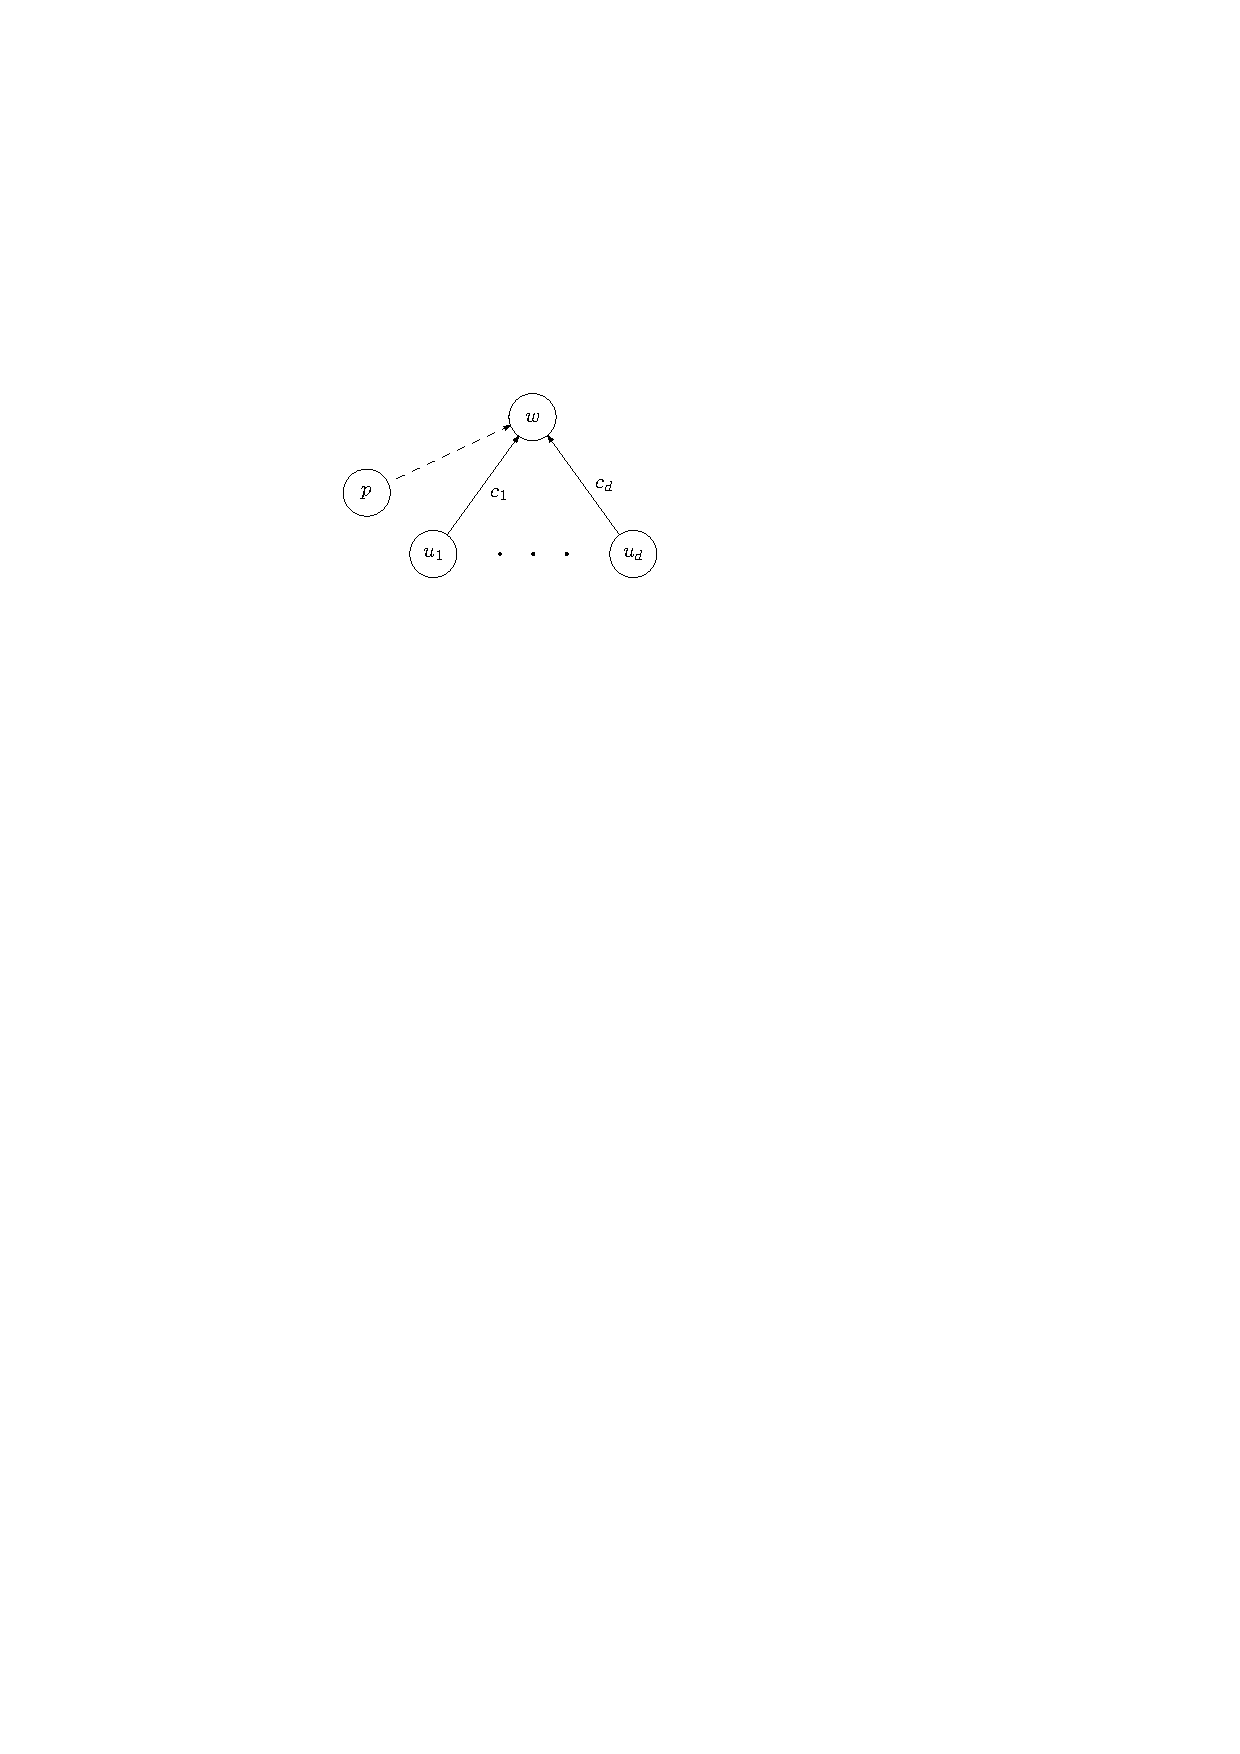
\includegraphics{figures/gsd-qs-triggered}
	\end{center}
	\caption{Illustration of the GSD graph when $\qs$ is triggered at a node $w$. The dashed edge represents a seed dependency $(p, w)$ and the remaining edges represent encryption queries $c_i \from \operatorname{encrypt}(u_i, w)$.}
	\label{fig:gsd-qs-triggered}
\end{figure}

The proof in \cite{ttkem} simply argued that this is not too likely if these encryptions were made with an IND-CPA secure scheme. In the context of the DHIES scheme we can say more about these encryptions and achieve a better reduction loss.
Let $(\mathbb{G}, q, g) = \mathcal{G}(1^\eta)$.
Let $x_i = \log_g(pk_{u_i})$. Each encryption $c_i$ is a tuple of the form $\langle g^{y_i}, \Pi_s.\enc_{k_i}(s_w) \rangle$ where $y_i \from [q], k_i = \hdh\left(g^{x_i \cdot y_i}\right)$. Now we can again do a case distinction on whether $\hdh$ was queried for (the encoding of) some group element $g^{x_j \cdot y_j}$ or not:
\begin{enumerate}[(i)]
	\item \label{qs-triggered-case-1} If such a query was made, then $\adv$ solved the Diffie-Hellman challenge $(g^{x_j}, g^{y_j})$. (Remember that we assumed that $w$ is the first node for which $\qs$ is triggered and as before if $w$ is safe, then so are the nodes $u_i$. Thus the adversary has not learned the exponent $x_i$ through querying $\hgen(s_{u_i})$ for any $i$.)
	\item \label{qs-triggered-case-2} If no such query was made, then from $\adv$'s perspective all the $k_i$ are independent, uniformly random keys and it still was able to learn $s_w$ from the EAV secure encryptions $\Pi_s.\enc_{k_1}(s_w), \ldots, \Pi_s.\enc_{k_d}(s_w)$.
\end{enumerate}
We can bound the probability of either of these events occurring using the hardness of the DDH problem relative to $\mathcal{G}$ and EAV security of $\Pi_s$, respectively.

To this end, we call a group element $h \in \mathbb{G}$ a \emph{hidden Diffie-Hellman key} if $h = pk_u^{y_{u, v}}$, where $(u, v)$ is an edge in the GSD graph, $u$ is safe and $y_{u, v}$ is the exponent chosen in the DHIES encryption of $s_v$ (i.e. $\adv$ was given a ciphertext of the form $\langle g^{y_{u, v}}, \ldots\rangle$ when it queried $\operatorname{encrypt}(u, v)$). Now analogously to above let $\qdh$ the event that $\adv$ queries $\hdh$ on a hidden Diffie-Hellman key, and let $\fdh$ the event that $\adv$ triggers $\qdh$ when $\qs$ has not (yet) been triggered.
\todo{Querying a hidden DH key can also happen when the adversary first queries the group element and then later does an encrypt query that creates an edge with that group element as the key. Add notes in SD-GSD adversaries in proofs to explain how they keep track of this and check if any arguments must be adapted (what is essential is that the adversary has not queried $\hdh(k)$ for any hidden key $k$ and the simulations are thus distributed identically).}
Then we can split the event $\qs$ into two cases as motivated above:
\begin{align*}
	\pr{\qs} & = \pr{\qs \land \fdh} + \pr{\qs \land \overline{\fdh}\,}.
\end{align*}
We bound $\pr{\qs \land \fdh}$ and $\pr{\qs \land \overline{\fdh} \,}$ in Lemma~\ref{lemma:dh-reduction} and Lemma~\ref{lemma:eav-reduction}, respectively.\footnote{To be precise, the event $\qs \land \fdh$ is a superset of case \ref{qs-triggered-case-1} above. However, the argument applied in Lemma~\ref{lemma:dh-reduction} gives the same bound for either event and this more general event has the advantage of being simpler.}
Overall this gives us a bound on the advantage of $\adv$ using \eqref{eq:theorem-sd-gsd-security-win-cases}.

\begin{proof}[of Theorem~\ref{theorem:sdgsd-security}]
	Let $\delta, N$ functions in $\eta$ (mapping to $\N$) with $\delta \le N$.
	Let $\eta$ arbitrary and let $\adv$ an arbitrary SD-GSD adversary constructing a GSD graph of size at most $N(\eta)$ and indegree at most $\delta(\eta)$, making at most $\ms(\eta)$ queries to $\hgen$ or $\hdep$ and at most $\mdh(\eta)$ queries to $\hdh$, each of length at most $\gamma(\eta)$, and running in time $\tilde{t}(\eta)$. We will use the events defined above.

	We first justify step $(\dagger)$ in \eqref{eq:theorem-sd-gsd-security-win-cases}. Note that by the rules imposed on the adversary in the SD-GSD game, the challenge node $v$ is safe and its seed is thus indeed hidden. If $\qdep$ does not hold, then $\adv$ has not queried $\hdep$ for $s_v$ and, by virtue of $\hdep$ being a random oracle, $\hdep(s_v)$ is a uniformly distributed value in $\{0, 1\}^\rho$ from $\adv$'s perspective. The value $s$ follows the same distribution. Thus, $\adv$ behaves the same when given either $r = s$ or $r = \hdep(s_v)$ and
	\begin{align} \label{eq:theorem-sd-gsd-security-not-qdep-behavior}
		\begin{split}
			\pr{1 \from \adv \mid \overline{\qdep}, b = 1} & = \pr{1 \from \adv \mid \overline{\qdep}, r = s}          \\
			& = \pr{1 \from \adv \mid \overline{\qdep}, r = \hdep(s_v)} \\
			& = \pr{1 \from \adv \mid \overline{\qdep}, b = 0}.
		\end{split}
	\end{align}
	Therefore
	\begin{align*}
		\pr{\wins \mid \overline{\qdep} \,} & = \begin{aligned}[t]
			                                         & \pr{1 \from \adv \mid \overline{\qdep}, b = 1} \cdot \frac{1}{2}   \\
			                                         & + \pr{0 \from \adv \mid \overline{\qdep}, b = 0} \cdot \frac{1}{2}
		                                        \end{aligned}                                                                             \\
		                                    & \stackrel{\mathclap{\eqref{eq:theorem-sd-gsd-security-not-qdep-behavior}}}{=} \begin{aligned}[t]
			                                                                                                                     & \pr{1 \from \adv \mid \overline{\qdep}, b = 0} \cdot \frac{1}{2}   \\
			                                                                                                                     & + \pr{0 \from \adv \mid \overline{\qdep}, b = 0} \cdot \frac{1}{2}
		                                                                                                                    \end{aligned} \\
		                                    & = \frac{1}{2}.
	\end{align*}

	By Lemma~\ref{lemma:dh-reduction} we have\footnote{Note that we are again omitting the argument $\eta$ from the functions on the right-hand side ($N, \eddh$ and $\mdh$ in this case).}
	\[
		\pr{\qs \land \fdh} \le N \cdot \eddh + \frac{\mdh \cdot N^2}{q}.
	\]
	and by Lemma~\ref{lemma:eav-reduction} we have
	\[
		\pr{\qs \land \overline{\fdh}\,} \le \delta \cdot N \cdot \eeav + \frac{\ms \cdot N}{2^\rho},
	\]
	so we know that
	\begin{equation} \label{eq:theorem-sd-gsd-security-qs-bound}
		\pr{\qs} \le N \cdot \eddh + \delta \cdot N \cdot \eeav + \frac{\mdh \cdot N^2}{q} + \frac{\ms \cdot N}{2^\rho} = \tilde{\epsilon}(\eta) / 2.
	\end{equation}
	Then
	\begin{align*}
		\advantage{\Pi}{\eta}{SD\text{-}GSD}(\adv) & = 2 \cdot \left(\pr{\wins} - \frac{1}{2}\right)                                                   \\
		                                    & \stackrel{\mathclap{\eqref{eq:theorem-sd-gsd-security-win-cases}}}{\le} \;  2 \cdot \pr{\qs}      \\
		                                    & \stackrel{\mathclap{\eqref{eq:theorem-sd-gsd-security-qs-bound}}}{\le} \; \tilde{\epsilon}(\eta).
	\end{align*}
\end{proof}

\subsubsection{Reducing to EAV security}

Recall case \ref{qs-triggered-case-2} in the high-level discussion of Theorem~\ref{theorem:sdgsd-security}: the adversary $\adv$ was able to learn the seed $s_w$ given the EAV secure encryptions $\Pi_s.\enc_{k_1}(s_w), \ldots, \Pi_s.\enc_{k_d}(s_w)$. We can see $\adv$ as an adversary in a security game where $\adv$ is given $d$ EAV secure encryptions $c_1 \from \Pi_s.\enc_{k_1}(m), \ldots, c_d \from \Pi_s.\enc_{k_d}(m)$ of a message $m$ with $k_i \from \Pi_s.\gen(1^\eta)$ and must compute $m$. If we can prove that beating such a game is hard, then we can bound the probability of $\adv$ actually learning $s_w$ in this way.

This is exactly how we proceed in this section. Instead of asking the adversary to compute an encrypted message $m$, we turn to a more familiar decisional formulation as in the IND-CPA game (where the adversary may choose a pair $m_0, m_1$ and must distinguish whether the $d$ ciphertexts encrypt $m_0$ or $m_1$). We call this security notion \emph{EAV security under multiple (M) independent (I) encryptions of a single (S) pair of messages} (MIS-EAV).

\begin{definition}[The MIS-EAV game]
	Let $\kappa$ denote the security parameter and let $\Pi$ a private-key encryption scheme. Define the game $\game{\Pi}{\kappa}{MIS-EAV}(\adv)$ for an adversary $\adv$:
	\begin{enumerate}[1.]
		\item The adversary $\adv$ outputs $q \in \N$ and a pair of messages $m_0, m_1$ of the same length. We refer to $q$ as the number of \emph{queries} made by $\adv$.
		\item A bit $b \from \{0, 1\}$ is sampled. For each $i \in [q]$, $\adv$ is given an encryption $c_i \from \Pi.\enc_{k_i}(m_b)$ where $k_i \from \Pi.\gen(1^\kappa)$ is generated independently of the other keys.
		\item $\adv$ outputs a bit $b'$. The output of the game is defined to be $1$ if $b' = b$, and $0$ otherwise.
	\end{enumerate}
\end{definition}

\begin{definition}[MIS-EAV security]
	A private-key encryption scheme $\Pi$ is \emph{$(t, \epsilon, q)$-MIS-EAV-secure} if for all $\kappa$, for any adversary $\adv$ making at most $q(\kappa)$ queries and running in time $t(\kappa)$ we have
	\begin{align*}
		\advantage{\Pi}{\kappa}{MIS-EAV}(\adv) \coloneqq 2 \cdot \left(\pr{\game{\Pi}{\kappa}{MIS-EAV}(\adv) = 1} - \frac{1}{2}\right) \le \epsilon(\kappa).
	\end{align*}
\end{definition}

Similar to how IND-CPA security for a single encryption query implies IND-CPA security for $q$ queries with a security loss of $q$ by a standard hybrid argument, one can show that EAV security implies MIS-EAV security with the same loss. To see why, recall the hybrid argument for IND-CPA security (as discussed in e.g. \cite[Theorem 12.6]{introduction-to-modern-cryptography}): We define the sequence of hybrid games $G_0, \ldots, G_q$ where in the game $G_i$ the first $i$ encryption queries encrypt the second message and the remaining $q - i$ queries encrypt the first message. Then given an IND-CPA adversary $\adv$ for multiple encryptions, an IND-CPA adversary $\adv'$ is constructed to bound
\[
	\abs*{\pr{\adv \text{ outputs } 0 \text{ in game } G_{i - 1}} - \pr{\adv \text{ outputs } 0 \text{ in game } G_{i}}}
\]
for arbitrary $i$.
The adversary $\adv'$ simulates $G_{i - 1}$ or $G_{i}$ to $\adv$ depending on whether the ciphertext received from the (single-query) IND-CPA challenger, which gets passed on as the response to the $i$-th query, encrypts the first or the second message from the $i$-th pair of messages. $\adv'$ then uses the encryption oracle to pass on the right encryptions to $\adv$ for all other queries. Now notice that if we wanted to simulate to an MIS-EAV adversary we would not need access to an encryption oracle since for the MIS-EAV security game all the other encryptions can easily be generated by $\adv'$ sampling the new keys itself.

The argument would of course also work without restricting the adversary to a single pair of messages (which we could call MI-EAV security). However, we will make use of this restriction to provide a tighter reduction for a certain class of schemes in the appendix.

\begin{lemma} \label{lemma:mis-eav-from-eav}
	Let $\Pi$ a private-key encryption scheme with finite message space. Let $t_{\gen}, t_{\enc}$ functions in $\kappa$ that upper bound the runtime of $\Pi.\gen$ and $\Pi.\enc$, respectively. If $\Pi$ is $(t, \epsilon)$-EAV-secure, then for any function $q$, $\Pi$ is $(\tilde{t}, q \cdot \epsilon, q)$-MIS-EAV-secure with $\tilde{t} = t - \mathcal{O}(q \cdot (t_\gen + t_\enc))$.
\end{lemma}

The details of the proof can be found in Section~\ref{sec:mis-eav-from-eav-proof} of the appendix.

\begin{lemma} \label{lemma:eav-reduction}
	Recall the assumptions, variables and events from the statement and proof of Theorem~\ref{theorem:sdgsd-security}. In particular, assume that $\Pi_s$ is $(t, \eeav)$-EAV-secure. Let $\eta$ arbitrary and let $\adv$ an SD-GSD adversary constructing a GSD graph of size at most $N(\eta)$ and indegree at most $\delta(\eta)$, making at most $\ms(\eta)$ queries to $\hgen$ or $\hdep$ and at most $\mdh(\eta)$ queries to $\hdh$, and running in time $\tilde{t}(\eta)$. Then
	\[
		\pr{\qs \land \overline{\fdh}\,} \le \delta \cdot N \cdot \eeav + \frac{\ms \cdot N}{2^\rho}.
	\]
\end{lemma}

\paragraph{Intuition} By Lemma~\ref{lemma:mis-eav-from-eav} we know that $\Pi_s$ is MIS-EAV secure. Continuing the high-level argument before the proof of Theorem~\ref{theorem:sdgsd-security}, consider the first moment that $\adv$ triggers $\qs \land \overline{\fdh}$ by querying the seed of some safe node $w$.  As intended, it follows from the definition of the event $\fdh$ that from $\adv$'s perspective all DHIES ciphertexts it got from queries $\operatorname{encrypt}(u, w)$ for any $u$ contain encryptions of $s_w$ under independent, uniformly random keys using $\Pi_s$. Moreover, as already argued once, $\adv$ has learned nothing from a potential seed dependency $(p, w)$, so these encryptions are everything $\adv$ had at its proposal to learn $s_w$.

We can use $\adv$'s ability to compute the seed $s_w$ of a safe node $w$ from encryptions of $s_w$ to construct an MIS-EAV adversary: We first guess a node $w$ whose seed $\adv$ may query first. Next, we give the MIS-EAV challenger $s_w$ and some other independent seed $s$. We simulate the SD-GSD game to $\adv$ and embed the encryptions from the MIS-EAV challenger when answering queries of the form $\operatorname{encrypt}(u, w)$ for any $u$. Now consider the behavior of $\adv$ depending on which seed the challenger chooses to encrypt:
\begin{itemize}
	\item If the challenger chooses to encrypt $s_w$, then $\adv$ will trigger the event $\qs \land \overline{\fdh}$ with the same probability as before. We can detect whether $\qs \land \overline{\fdh}$ gets triggered since all seeds in the simulation are known. If $\qs \land \overline{\fdh}$ occurs and we guessed $w$ correctly, the event will be triggered at $w$ and $\adv$ will query $s_w$, telling us that the challenger encrypted $s_w$.
	\item If the challenger chooses to encrypt $s$, then $\adv$ receives no information about $s_w$ and has a negligible probability of querying it.
\end{itemize}
Thus, the advantage of the MIS-EAV adversary is about $\pr{\qs \land \overline{\fdh}\,}/N$, where the factor $1/N$ arises from guessing $w$, and using that $\Pi_s$ is MIS-EAV secure we can bound this probability. Since we are only interested in checking whether the event was triggered for $w$, the adversary can abort when this is no longer possible ($w$ is corrupted, some other hidden seed is queried, etc.). The details of the proof can be found in Section~\ref{sec:eav-reduction-proof} of the appendix.

For a certain class of schemes, we can improve on Lemma~\ref{lemma:mis-eav-from-eav} and achieve a tight reduction. This allows us to get rid of the factor $\delta$ in Lemma~\ref{lemma:eav-reduction}. However, we do not use this in our main result and refer the interested reader to Section~\ref{sec:tighter-mis-eav-security} of the appendix.

\subsubsection{Reducing to the DDH problem}

\begin{lemma} \label{lemma:dh-reduction}
	Recall the assumptions, variables and events from the statement and proof of Theorem~\ref{theorem:sdgsd-security}. In particular, assume that the DDH problem is $(t, \eddh)$-hard relative to $\mathcal{G}$. Let $\eta$ arbitrary and let $\adv$ an SD-GSD adversary constructing a GSD graph of size at most $N(\eta)$ and indegree at most $\delta(\eta)$, making at most $\ms(\eta)$ queries to $\hgen$ or $\hdep$ and at most $\mdh(\eta)$ queries to $\hdh$, and running in time $\tilde{t}(\eta)$. Then
	\[
		\pr{\qs \land \fdh} \le N \cdot \eddh + \frac{\mdh \cdot N^2}{q}.
	\]
\end{lemma}

\paragraph{Intuition} We will bound the simpler event $\fdh$. This event tells us that there is some safe node $a$ in the GSD graph with encryption edges to nodes $u_1, \ldots, u_d$, where the query $\operatorname{encrypt}(a, u_i)$ returned the ciphertext $\langle g^{y_i}, \Pi_s.\enc_{k_i}(s_{u_i}) \rangle$ with $k_i = \hdh(g^{sk_{a} \cdot y_i})$, such that $g^{sk_a \cdot y_j}$ was the first hidden Diffie-Hellman key queried by $\adv$ for some $j$.
Moreover, at the time $g^{sk_a \cdot y_j}$ was queried, no hidden seed had yet been queried by $\adv$, implying that $\adv$ had not queried $\hgen(s_a)$ and thus had no information about $sk_a$ besides $pk_a$ (recall that $(pk_a, sk_a) = \dhies.\gen(1^\eta, \hgen(s_a))$).

It is interesting to note that our approach does not require that $\adv$ has not queried $\hdep$ for a hidden seed (i.e. that $\qdep$ was not triggered) as is implied by the event $\fdh$, because knowing $\hgen(s_a)$ is the only way to learn about $sk_a$. Regardless, we still want to have our definition of $\fdh$ include this information, as the bound on $\pr{\qs \land \overline{\fdh} \,}$ in Lemma~\ref{lemma:eav-reduction} relies on the fact that in the event of $\qs \land \overline{\fdh}$ happening,  $\qdh$ was not yet triggered when the event $\qs$ was triggered, i.e. when either the event $\qgen$ \emph{or} the event $\qdep$ was triggered.

The intuition is clear that this means that $\adv$ solved the Diffie-Hellman challenge $(g^{sk_a}, g^{y_j})$. What is not immediately clear is how to embed a \emph{given} Diffie-Hellman challenge $(g^x, g^y)$ from an instance of the DDH game and use $\adv$ to tell whether the key $k$ chosen by the challenger is the real key $g^{x \cdot y}$ or a uniformly random group element.
An intuitive strategy would be to embed the challenge by setting $pk_a = g^x$ and $g^{y_j} = g^y$, which involves guessing $u_j$, and simply checking whether for any of the queries $q_i$ to $\hdh$ by $\adv$, such that $q_i$ encodes a group element in $\mathbb{G}$, it holds that $q_i = k$. Now:
\begin{itemize}
	\item If $k = g^{x \cdot y}$, $\adv$ triggers $\fdh$ and we guessed $a$ and $u_j$ correctly, then indeed as described above $q_i = g^{sk_a \cdot y_j} = g^{x \cdot y} = k$ will hold for some $i$.
	\item If $k$ is a random group element, then $\adv$ has negligible probability of querying $k$, as no information about $k$ is ever leaked to $\adv$.
\end{itemize}
If we make sure not to change $\adv$'s view of the game in the case $k = g^{x \cdot y}$ in this process, we can achieve an advantage of about $\pr{\fdh} / N^2$, where one factor $1/N$ arises from guessing $a$ and another from guessing $u_j$. Unfortunately, this would yield no improvement over the result from \cite{ttkem}.

To avoid this issue, we can use the random self-reducibility of the DDH problem and avoid guessing $u_j$. Instead of embedding $g^y$ into a single encryption edge, we embed it into all $d$ encryption edges. To get a uniformly random exponent from $y$ we set $y_j = y + r_j \mod q$ with $r_j \from [q]$. Given $g^{x \cdot y_j}$, we can easily compute $g^{x \cdot y}$:
\[
	g^{x \cdot y_j} = g^{x \cdot (y + r_j)} = g^{x \cdot y}	\cdot g^{x \cdot r_j} \iff g^{x \cdot y} = g^{x \cdot y_j} \cdot \underbrace{((g^x)^{r_j})^{-1}}_{\eqqcolon \, R_j}.
\]
Now to determine whether $k$ is the real Diffie-Hellman key, we check whether $q_i \cdot R_j = k$ for some $i, j$. This yields an advantage of about $\pr{\fdh} / N$ (and a slightly larger runtime). The details of the proof can be found in Section~\ref{sec:dh-reduction-proof} of the appendix.
